 
\chapter{Normal Linear Model: Inference and Prediction}
 \label{chapter::normal-linear-model}


Under the Gauss--Markov model, we have calculated the first two moments of the OLS estimator $\hat{\beta} = (X^{\T} X)^{-1} X^{\T} Y$:
\begin{eqnarray*}
E(\hat{\beta}) &=& \beta,\\
\cov(\hat{\beta}) &=& \sigma^{2}(X^{\T}X)^{-1},
\end{eqnarray*}
and have shown that $\hat{\sigma}^{2} =   \hat{\varepsilon}^{\T}  \hat{\varepsilon} / (n-p)$ is unbiased for $\sigma^{2}$, where $\hat{\varepsilon} = Y - X \hat{\beta}$ is the residual vector. The Gauss--Markov theorem further ensures that the OLS estimator is BLUE. 
Although these results characterize the nice properties of the OLS estimator,
they do not fully determine its distribution and are thus inadequate
for statistical inference.

 This chapter will derive the joint distribution
of $(\hat{\beta},\hat{\sigma}^{2})$ under the Normal linear model with stronger distribution assumptions. 

 

\begin{assumption}
[Normal linear model] 
\label{assume::nlm}
We have
$$
Y\sim\N(X\beta,\sigma^{2}I_{n}) , 
$$
or, equivalently,
$$
y_{i} \stackrel{ \textsc{ind} }{ \sim}\N(x_{i}^{\T}\beta,\sigma^{2}),\qquad(i=1,\ldots,n),
$$ 
where the design matrix $X$ is fixed with linearly independent column vectors. The unknown parameters are $(\beta,\sigma^{2})$. 
\end{assumption}

We can also write the Normal linear model as a linear function of covariates with error terms:
$$
Y = X\beta +\varepsilon 
$$
or, equivalently, 
$$
y_i = x_{i}^{\T}\beta  +\varepsilon_i,\qquad(i=1,\ldots,n),
$$
where 
$$
\varepsilon \sim \N(0,\sigma^2 I_n) \text{ or } \varepsilon_i \iidsim \N(0,\sigma^2), \qquad(i=1,\ldots,n). 
$$ 


Assumption \ref{assume::nlm} implies Assumption \ref{assume::gm-model}. Beyond the Gauss--Markov model, it further requires IID Normal error terms. 
Assumption \ref{assume::nlm} is extremely strong, but it is canonical in statistics. It allows us to derive elegant formulas and also justifies the outputs of the linear regression functions in many statistical packages. I will relax it in Chapter \ref{chapter::EHW}. 


\section{Joint distribution of the OLS coefficient and variance estimator}
% $(\hat{\beta},\hat{\sigma}^{2})$}

We first state the main theorem on the joint distribution of $(\hat{\beta},\hat{\sigma}^{2})$
via the joint distribution of $(\hat{\beta},\hat{\varepsilon}).$
\begin{theorem}
\label{thm:normalexactdistribution}Under Assumption \ref{assume::nlm}, we have 
\[
\left(\begin{array}{c}
\hat{\beta}\\
\hat{\varepsilon}
\end{array}\right)\sim\N\left\{ \left(\begin{array}{c}
\beta\\
0
\end{array}\right),\sigma^{2}\left(\begin{array}{cc}
(X^{\T}X)^{-1} & 0\\
0 & I_{n}-H
\end{array}\right)\right\} ,
\]
and
$$
\hat{\sigma}^{2}/\sigma^{2}\sim\chi_{n-p}^{2}/(n-p).
$$
So 
$$
\hat{\beta}\ind\hat{\varepsilon} ,\quad 
 \hat{\beta}\ind\hat{\sigma}^{2}  .
$$
\end{theorem}
 
\begin{myproof}{Theorem}{\ref{thm:normalexactdistribution}}
First, 
\begin{eqnarray*}
\left(\begin{array}{c}
\hat{\beta}\\
\hat{\varepsilon}
\end{array}\right)
&=&
\left(\begin{array}{c}
(X^{\T}X)^{-1}X^{\T}Y\\
(I_{n}-H)Y
\end{array}\right) \\
&=&\left(\begin{array}{c}
(X^{\T}X)^{-1}X^{\T}\\
I_{n}-H
\end{array}\right)Y
\end{eqnarray*}
is a linear transformation of $Y$, so they are jointly Normal. We have verified their means and variances in Chapter \ref{chapter::gauss-markov}, so we only need to show that their covariance is zero:
\begin{eqnarray*}
\cov(\hat{\beta},\hat{\varepsilon})
&=&(X^{\T}X)^{-1}X^{\T}\cov(Y)(I_{n}-H)^{\T}\\
&=&\sigma^{2}(X^{\T}X)^{-1}X^{\T}(I_{n}-H^{\T}) \\
&=&0
\end{eqnarray*}
which holds because $(I_{n}-H)X=0$ by Lemma \ref{lem:projectionms}.

 

Second, because $\hat{\sigma}^{2}=\textsc{rss}/(n-p)=\hat{\varepsilon}^{\T}\hat{\varepsilon}/(n-p)$
is a quadratic function of $\hat{\varepsilon}$, it is independent
of $\hat{\beta}$. We only need to show that it is a scaled chi-squared
distribution. This follows from Theorem \ref{thm::normal-chisq} in Chapter \ref{chapter:appendix-rvs}  due to the Normality of $\hat{\varepsilon}/\sigma$
with the projection matrix $I_{n}-H$ as its covariance matrix. 
\end{myproof}



The second theorem is on the joint distribution of $(\hat{Y},\hat{\varepsilon}).$
We have shown their means and covariance matrix in the last chapter.
Because they are linear transformations of $Y$, they are jointly Normal
and independent. 
\begin{theorem}\label{thm::gaussianlm-independence-ye}
Under Assumption \ref{assume::nlm}, we have 
\[
\left(\begin{array}{c}
\hat{Y}\\
\hat{\varepsilon}
\end{array}\right)\sim\N\left\{ \left(\begin{array}{c}
X\beta\\
0
\end{array}\right),\sigma^{2}\left(\begin{array}{cc}
H & 0\\
0 & I_{n}-H
\end{array}\right)\right\} ,
\]
so 
$$
\hat{Y}\ind\hat{\varepsilon}.
$$
\end{theorem}
 

Recall that we have shown that $Y = \hat{Y}  + \hat{\varepsilon}$ with $\hat{Y}  \perp  \hat{\varepsilon}$ by the OLS properties, which is a pure linear algebra fact without assumptions.
Theorem \ref{thm:GMcov} ensures that $\hat{Y} $ and $  \hat{\varepsilon}$ are uncorrelated under Assumption \ref{assume::gm-model}.
Now Theorem \ref{thm::gaussianlm-independence-ye} further ensures that $\hat{Y}  \ind  \hat{\varepsilon}$ under Assumption \ref{assume::nlm}. The first result states that $\hat{Y} $ and $  \hat{\varepsilon}$
are orthogonal. The second result states that $\hat{Y} $ and $  \hat{\varepsilon}$ are uncorrelated. The third result states $\hat{Y} $ and $  \hat{\varepsilon}$ are independent. They hold under different assumptions. 



\section{Pivotal quantities and statistical inference}

\subsection{Scalar parameters}
We first consider statistical inference for $c ^{\T}\beta$,
a one-dimensional linear function of $\beta$ where $c \in\mathbb{R}^{p}.$
For example, if $c = e_j \equiv   (0,\ldots,1,\ldots,0)^{\T}$ with only the
$j$th element being one, then $c ^{\T}\beta=\beta_{j}$ is the
$j$th element of $\beta$ which measures the impact of $x_{ij}$
on $y_{i}$ on average. Standard software packages report statistical
inference for each element of $\beta$. Sometimes we may also be interested in $\beta_j - \beta_{j'}$, the difference between the coefficients of two covariates, which corresponds to $c=(0, \ldots,0,1,0,\ldots,0,-1,0,\ldots,0)^{\T} = e_j - e_{j'}$. 

Theorem \ref{thm:normalexactdistribution} implies that 
\[
c ^{\T}\hat{\beta}\sim\N\left\{ c ^{\T}\beta,\sigma^{2}c ^{\T}(X^{\T}X)^{-1}c \right\} .
\]
However, this is not directly useful because $\sigma^{2}$ is unknown.
With $\sigma^{2}$ replaced by $\hat{\sigma}^{2}$, the standardized
distribution
\[
T_c \equiv 
\frac{c ^{\T}\hat{\beta}-c ^{\T}\beta}{\sqrt{\hat{\sigma}^{2}c ^{\T}(X^{\T}X)^{-1}c }}
\]
does not follow $\N(0,1)$ anymore. In fact, it is a $t$ distribution as shown in Theorem \ref{thm:1dimpivotal} below. 

\begin{theorem}
\label{thm:1dimpivotal}Under Assumption \ref{assume::nlm}, for a fixed vector $c  \in \mathbb{R}^p$, we have 
$$
T_c  \sim t_{n-p}.
$$
\end{theorem}


\begin{myproof}{Theorem}{\ref{thm:1dimpivotal}}
From Theorem \ref{thm:normalexactdistribution}, the standardized
distribution with the true $\sigma^{2}$ follows
\[
\frac{c ^{\T}\hat{\beta}-c ^{\T}\beta}{\sqrt{\sigma^{2}c ^{\T}(X^{\T}X)^{-1}c }}\sim\N(0,1),
\]
 $\hat{\sigma}^{2}/\sigma^{2}\sim\chi_{n-p}^{2}/(n-p),$ and they
are independent. These facts imply that
\begin{align*}
T_c &= 
\frac{c ^{\T}\hat{\beta}-c ^{\T}\beta}{\sqrt{\hat{\sigma}^{2}c ^{\T}(X^{\T}X)^{-1}c }} \\
& =\frac{c ^{\T}\hat{\beta}-c ^{\T}\beta}{\sqrt{\sigma^{2}c ^{\T}(X^{\T}X)^{-1}c }}\Big/\sqrt{\frac{\hat{\sigma}^{2}}{\sigma^{2}}}\\
 & \sim \frac{\N(0,1)}{\sqrt{\chi_{n-p}^{2}/(n-p)}} ,
\end{align*}
where $\N(0,1)$ and $\chi_{n-p}^{2}$ denote independent standard Normal and $\chi_{n-p}^{2}$ random variables, respectively, with a little abuse of notation. Therefore, 
$T_c \sim t_{n-p}$ by the definition of the $t$ distribution. 
\end{myproof}



In Theorem \ref{thm:1dimpivotal}, the left-hand side
depends on the observed data and the unknown true parameters, but the
right-hand side is a random variable depending on only the dimension
$(n,p)$ of $X$, but neither the data nor the true parameters. We
call the quantity on the left-hand side a {\it pivotal quantity}. Based
on the quantiles of the $t_{n-p}$ random variable, we can tie the
data and the true parameter via the following probability statement
\[
\pr\left\{ \left|\frac{c ^{\T}\hat{\beta}-c ^{\T}\beta}{\sqrt{\hat{\sigma}^{2}c ^{\T}(X^{\T}X)^{-1}c }}\right|\leq  
t_{1-\alpha/2,n-p}
\right\} =1-\alpha
\]
 for any $0<\alpha<1$, where $t_{1-\alpha/2,n-p}  $ is the $1-\alpha/2$
quantile of $t_{n-p}$. 
When $n-p$ is large (e.g. larger than $30$), the $1-\alpha/2$ quantile of $t_{n-p}$ is close to that of $\N(0,1)$. 
In particular,  $t_{97.5\%,n-p}\approx 1.96$, the $97.5\%$ quantile of $\N(0,1)$, which is the critical value for the $95\%$ confidence interval. 


Define 
$$
\sqrt{\hat{\sigma}^{2}c ^{\T}(X^{\T}X)^{-1}c }\equiv \hat{\text{se}}_{c }
$$
which is often called the (estimated) standard error of $c ^{\T}\hat{\beta}$. Using this definition,
we can equivalently write the above probability statement as
\[
\pr\left\{ c ^{\T}\hat{\beta}- t_{1-\alpha/2,n-p} \hat{\text{se}}_{c }\leq c ^{\T}\beta\leq c ^{\T}\hat{\beta}+ t_{1-\alpha/2,n-p} \hat{\text{se}}_{c }\right\} =1-\alpha.
\]
We use 
\[
c ^{\T}\hat{\beta} \pm t_{1-\alpha/2,n-p} \hat{\text{se}}_{c } 
\]
as a $1-\alpha$ level confidence interval for $c ^{\T}\beta$. By duality of confidence
interval and hypothesis testing, we can also construct a level $\alpha$
test for $c ^{\T}\beta$. More precisely, we reject the null hypothesis $c ^{\T}\beta = d$ if the above confidence interval does not cover $d$, for a fixed number $d$. 


As an important case, $c=e_j$ so $c^{\T} \beta = \beta_j$. Standard software packages, for example, \ri{R}, report the point estimator $\hat{\beta}_j$, the standard error $\hat{\text{se}}_j = \sqrt{ \hat{\sigma}^2 [(X^{\T}X)^{-1}]_{jj} }$, the $t$ statistic $T_j = \hat{\beta}_j / \hat{\text{se}}_j $, and the two-sided $p$-value $\pr( | t_{n-p} | \geq  |T_j|  )$ for testing whether $\beta_j$ equals zero or not. Section \ref{sec::normallinearmodel-r} below gives some examples. 



\subsection{Vector parameters}
We then consider statistical inference for $C\beta$, a multi-dimensional
linear function of $\beta$ where $C\in\mathbb{R}^{l\times p}.$ If
$l=1$, then it reduces to the one-dimensional case. If $l>1$, then 
$$
C = \begin{pmatrix}
c_1^{\T} \\
\vdots \\
c_l^{\T}
\end{pmatrix} \Longrightarrow 
C\beta = \begin{pmatrix}
c_1^{\T} \beta \\
\vdots \\
c_l^{\T} \beta
\end{pmatrix}
$$
correspond to the joint value of $l$ parameters $ c_1^{\T} \beta, \ldots,c_l^{\T} \beta$.

\begin{example}\label{eg::testing-1}
If
\[
C=\left(\begin{array}{ccccc}
0 & 1 & 0 & \cdots & 0\\
0 & 0 & 1 & \cdots & 0\\
\vdots & \vdots & \vdots & \cdots & \vdots\\
0 & 0 & 0 & \cdots & 1
\end{array}\right) , 
\]
then 
\[
C\beta=\left(\begin{array}{c}
\beta_{2}\\
\vdots\\
\beta_{p}
\end{array}\right),
\]
contains all the coefficients except for the first one (the
intercept in most cases). Most software packages report the test of
the joint significance of $(\beta_{2}, \ldots, \beta_{p})$. Section \ref{sec::normallinearmodel-r} below gives some examples. 
\end{example}

\begin{example}\label{eg::partition-reg-F}
Another
leading application is to test whether $\beta_{2}=0$ in the following
regression partitioned by $X=(X_{1},X_{2})$ where $X_{1}$ and $X_{2}$
are $n\times k$ and $n\times l$ matrices:
\[
Y=X_{1}\beta_{1}+X_{2}\beta_{2}+\varepsilon,
\]
 with
\[
C=\left(\begin{array}{cc}
0_{l\times k} & I_{l}\end{array}\right)\left(\begin{array}{c}
\beta_{1}\\
\beta_{2}
\end{array}\right)\Longrightarrow C\beta=\beta_{2}.
\]
 We will discuss this partitioned regression in more detail in Chapters \ref{chapter::FWL-theorem} and \ref{chapter::FWL-application}.
 \end{example}
 
Now we will focus on the generic problem of inferring $C\beta$.
To avoid degeneracy, we assume that $C$ does not have redundant rows, quantified below. 

\begin{assumption}\label{assume::c-non-degenerate}
 $C$ has linearly independent
rows. 
\end{assumption}


Theorem \ref{thm:normalexactdistribution} implies that 
\[
C\hat{\beta}-C\beta\sim\N\left\{ 0,\sigma^{2}C(X^{\T}X)^{-1}C^{\T}\right\} 
\]
and therefore the standardized quadratic form has a chi-squared distribution
\[
(C\hat{\beta}-C\beta)^{\T}\left\{ \sigma^{2}C(X^{\T}X)^{-1}C^{\T}\right\} ^{-1}(C\hat{\beta}-C\beta)\sim\chi_{l}^{2}.
\]
The above chi-squared distribution follows from the property of the quadratic form of a Normal in Theorem \ref{thm::normal-chisq}, where $\sigma^{2}C(X^{\T}X)^{-1}C^{\T}$ is a positive definite matrix\footnote{Because $X$ has linearly independent columns, $X^{\T}X$ is a non-degenerate and thus positive definite
matrix. Since $ u^{\T} C(X^{\T}X)^{-1}C^{\T}u \geq 0$, to show that $C(X^{\T}X)^{-1}C^{\T}$ is non-degenerate, we only need to show that 
$$
u^{\T} C(X^{\T}X)^{-1}C^{\T}u  = 0  \Longrightarrow u = 0. 
$$
From $u^{\T} C(X^{\T}X)^{-1}C^{\T}u  = 0$, we know  $C^{\T}u = u_1 c_1 + \cdots u_l c_l = 0$. Since the rows of $C$ are linearly independent, we must have $u = 0$. }.
Again this is not directly useful with unknown $\sigma^{2}.$ Replacing
$\sigma^{2}$ with the unbiased estimator $\hat{\sigma}^{2}$ and
using a scaling factor $l$, we can obtain a pivotal quantity that
has an $F$ distribution as summarized in  Theorem \ref{thm:ldimpivotal} below.

\begin{theorem}
\label{thm:ldimpivotal}Under Assumptions \ref{assume::nlm} and \ref{assume::c-non-degenerate}, we have 
\[
F_C \equiv 
\frac{(C\hat{\beta}-C\beta)^{\T}\left\{ C(X^{\T}X)^{-1}C^{\T}\right\} ^{-1}(C\hat{\beta}-C\beta)}{l\hat{\sigma}^{2}}\sim F_{l,n-p}.
\]
\end{theorem}


\begin{myproof}{Theorem}{\ref{thm:ldimpivotal}}
Similar to the proof of Theorem \ref{thm:1dimpivotal}, we apply Theorem
\ref{thm:normalexactdistribution} to derive that
\[
\begin{aligned} 
F_C
= & \frac{(C\hat{\beta}-C\beta)^{\T}\left\{ \sigma^{2}C(X^{\T}X)^{-1}C^{\T}\right\} ^{-1}(C\hat{\beta}-C\beta)/l}{\hat{\sigma}^{2}/\sigma^{2}}\\
\sim & \frac{\chi_{l}^{2}/l}{\chi_{n-p}^{2}/(n-p)} ,
\end{aligned}
\]
where $\chi_{l}^{2} $ and $\chi_{n-p}^{2} $ denote independent $\chi_{l}^{2} $ and $\chi_{n-p}^{2} $ random variables, respectively, with a little abuse of notation. Therefore, $F_C  \sim  F_{l,n-p}$ by the definition of the $F$ distribution. 
\end{myproof}



Theorem \ref{thm:ldimpivotal} motivates the following confidence
region for $C\beta$:
\[
\left\{ r  :(C\hat{\beta}- r )^{\T}\left\{ C(X^{\T}X)^{-1}C^{\T}\right\} ^{-1}(C\hat{\beta}- r)\leq l\hat{\sigma}^{2}
f_{1-\alpha, l, n-p}
\right\} ,
\]
 where $f_{1-\alpha, l, n-p}$ is the upper $\alpha$ quantile of the
$F_{l,n-p}$ distribution. By duality of the confidence region and hypothesis
testing, we can also construct a level $\alpha$ test for $C\beta$. Most statistical packages automatically report the $p$-value based on the $F$ statistic in Example \ref{eg::testing-1}. 
 

As a final remark, the statistics in Theorems \ref{thm:1dimpivotal}
and \ref{thm:ldimpivotal} are called the Wald-type statistics. 

\section{Prediction based on pivotal quantities}\label{sec::prection-normallinear}

Practitioners use OLS not only to infer $\beta$ but also to predict
future outcomes. For the pair of future data $(x_{n+1},y_{n+1})$, we observe
only $x_{n+1}$ and want to predict $y_{n+1}$ based on $(X,Y)$ and $x_{n+1}$.
Assume a stable relationship between $y_{n+1}$ and $x_{n+1}$, that is,
\[
y_{n+1}\sim\N(x_{n+1}^{\T}\beta,\sigma^{2})
\]
with the same $(\beta,\sigma^{2}).$ 

First, we can predict the mean of $y_{n+1}$ which is $x_{n+1}^{\T}\beta$.
It is just a one-dimensional linear function of $\beta$, so the theory
in Theorem \ref{thm:1dimpivotal} is directly applicable. A natural
unbiased predictor is $x_{n+1}^{\T}\hat{\beta}$ with $1-\alpha$ level
prediction interval
\[
 x_{n+1}^{\T}\hat{\beta} \pm t_{1-\alpha/2,  n-p} \hat{\text{se}}_{x_{n+1}} .
\]

Second, we can predict $y_{n+1}$ itself, which is a random variable.
We can still use $x_{n+1}^{\T}\hat{\beta}$ as a natural unbiased predictor
but need to modify the prediction interval. Because $y_{n+1}\ind\hat{\beta}$,
we have
\[
y_{n+1}-x_{n+1}^{\T}\hat{\beta}\sim\N\left\{ 0,\sigma^{2}+\sigma^{2}x_{n+1}^{\T}(X^{\T}X)^{-1}x_{n+1}\right\} ,
\]
and therefore
\begin{align*}
\frac{y_{n+1}-x_{n+1}^{\T}\hat{\beta}}{\sqrt{\hat{\sigma}^{2}+\hat{\sigma}^{2}x_{n+1}^{\T}(X^{\T}X)^{-1}x_{n+1}}} & =\frac{y_{n+1}-x_{n+1}^{\T}\hat{\beta}}{\sqrt{\sigma^{2}+\sigma^{2}x_{n+1}^{\T}(X^{\T}X)^{-1}x_{n+1}}}\Big/\sqrt{\frac{\hat{\sigma}^{2}}{\sigma^{2}}}\\
 & \sim\frac{\N(0,1)}{\sqrt{\chi_{n-p}^{2}/(n-p)}} , 
\end{align*}
where $\N(0,1)$ and $\chi_{n-p}^{2}$ denote independent standard Normal and $\chi_{n-p}^{2}$ random variables, respectively, with a little abuse of notation. Therefore,  
$$
\frac{y_{n+1}-x_{n+1}^{\T}\hat{\beta}}{\sqrt{\hat{\sigma}^{2}+\hat{\sigma}^{2}x_{n+1}^{\T}(X^{\T}X)^{-1}x_{n+1}}}
  \sim t_{n-p}
$$
is a pivotal quantity. Define  the squared prediction error  as
\begin{align*}
\hat{\text{pe}}_{x_{n+1}}^{2} & =\hat{\sigma}^{2}+\hat{\sigma}^{2}x_{n+1}^{\T}(X^{\T}X)^{-1}x_{n+1}\\
 & =\hat{\sigma}^{2}\left\{ 1+n^{-1}x_{n+1}^{\T}\left(n^{-1}\sumn x_{i}x_{i}^{\T}\right)^{-1}x_{n+1}\right\}  ,
\end{align*}
which has two components. The first one has magnitude close to $\sigma^{2}$
which is of constant order. The second one has a magnitude decreasing
in $n$ if $n^{-1}\sumn x_{i}x_{i}^{\T}$ converges to a finite limit
with large $n$. Therefore, the first component dominates the second
one with large $n$, which results in the main difference between
predicting the mean of $y_{n+1}$ and predicting $y_{n+1}$ itself. Using
the notation $\hat{\text{pe}}_{x_{n+1}}$, we can construct the following
$1-\alpha$ level prediction interval: 
\[
 x_{n+1}^{\T}\hat{\beta} \pm  t_{1-\alpha/2,  n-p} \hat{\text{pe}}_{x_{n+1}} .
\]


\section{Examples and \ri{R} implementation}
\label{sec::normallinearmodel-r}


Below I illustrate the theory in this chapter with two classic datasets. 


\subsection{Univariate regression}


Revisiting Galton's data, we have the following result: 

\begin{lstlisting}
> library("HistData")
> galton_fit = lm(childHeight ~ midparentHeight,
+                 data = GaltonFamilies)
> round(summary(galton_fit)$coef, 3)
                Estimate Std. Error t value Pr(>|t|)
(Intercept)       22.636      4.265   5.307        0
midparentHeight    0.637      0.062  10.345        0
\end{lstlisting}


With the fitted line, we can predict \ri{childHeight} at different values of \ri{midparentHeight}. In the \ri{predict} function, if we specify \ri{interval = "confidence"}, it gives the {\it confidence} intervals for the means of the new outcomes; if we specify \ri{interval = "prediction"}, it gives the {\it prediction} intervals for the new outcomes themselves. 

\begin{lstlisting}
> new_mph  = seq(60, 80, by = 0.5)
> new_data = data.frame(midparentHeight = new_mph)
> new_ci   = predict(galton_fit, new_data, 
+                    interval = "confidence")
> new_pi   = predict(galton_fit, new_data, 
+                    interval = "prediction")
> round(head(cbind(new_ci, new_pi)), 3)
     fit    lwr    upr    fit    lwr    upr
1 60.878 59.744 62.012 60.878 54.126 67.630
2 61.197 60.122 62.272 61.197 54.454 67.939
3 61.515 60.499 62.531 61.515 54.782 68.249
4 61.834 60.877 62.791 61.834 55.109 68.559
5 62.153 61.254 63.051 62.153 55.436 68.869
6 62.471 61.632 63.311 62.471 55.762 69.180
\end{lstlisting}



Figure \ref{fig::prediction-galton} plots the fitted line as well as the confidence intervals and prediction intervals at level $95\%$.  The file \ri{code5.4.1.R} contains the  \ri{R} code. 

\begin{figure}[ht]
\centering
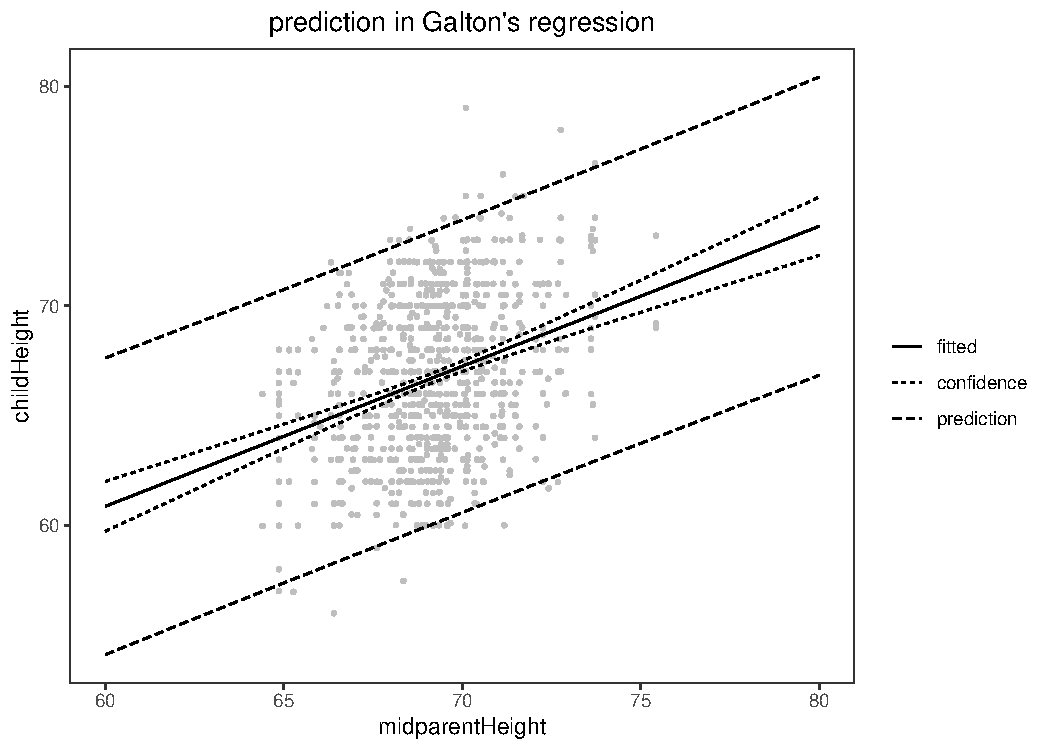
\includegraphics[width = \textwidth]{figures/galton_prediction_ggplot.pdf}
\caption{Prediction in Galton's regression}\label{fig::prediction-galton}
\end{figure}


\subsection{Multivariate regression}\label{section::normal-lm-lalonde}


The \ri{R} package \ri{Matching} contains an experimental dataset \ri{lalonde} from \citet{lalonde1986evaluating}. Units were randomly assigned to the job training program, with \ri{treat} being the treatment indicator. The outcome \ri{re78} is the real earnings in 1978, and other variables are pretreatment covariates. From the simple OLS, the treatment has a significant positive effect, whereas none of the covariates are predictive of the outcome. 


\begin{lstlisting}
> library("Matching")
> data(lalonde)
> lalonde_fit = lm(re78 ~ ., data = lalonde)
> summary(lalonde_fit)

Call:
lm(formula = re78 ~ ., data = lalonde)

Residuals:
   Min     1Q Median     3Q    Max 
 -9612  -4355  -1572   3054  53119 

Coefficients:
              Estimate Std. Error t value Pr(>|t|)   
(Intercept)  2.567e+02  3.522e+03   0.073  0.94193   
age          5.357e+01  4.581e+01   1.170  0.24284   
educ         4.008e+02  2.288e+02   1.751  0.08058 . 
black       -2.037e+03  1.174e+03  -1.736  0.08331 . 
hisp         4.258e+02  1.565e+03   0.272  0.78562   
married     -1.463e+02  8.823e+02  -0.166  0.86835   
nodegr      -1.518e+01  1.006e+03  -0.015  0.98797   
re74         1.234e-01  8.784e-02   1.405  0.16079   
re75         1.974e-02  1.503e-01   0.131  0.89554   
u74          1.380e+03  1.188e+03   1.162  0.24590   
u75         -1.071e+03  1.025e+03  -1.045  0.29651   
treat        1.671e+03  6.411e+02   2.606  0.00948 **

Residual standard error: 6517 on 433 degrees of freedom
Multiple R-squared:  0.05822,	Adjusted R-squared:  0.0343 
F-statistic: 2.433 on 11 and 433 DF,  p-value: 0.005974
\end{lstlisting}



The above result shows that none of the pretreatment covariates is significant. It is also of interest to test whether they are jointly significant. The result below shows that they are only marginally significant at the level $0.05$ based on a joint test. 

\begin{lstlisting}
> library("car")
> linearHypothesis(lalonde_fit,
+                  c("age=0", "educ=0", "black=0",
+                    "hisp=0", "married=0", "nodegr=0",
+                    "re74=0", "re75=0", "u74=0",
+                    "u75=0"))
Linear hypothesis test

Hypothesis:
age = 0
educ = 0
black = 0
hisp = 0
married = 0
nodegr = 0
re74 = 0
re75 = 0
u74 = 0
u75 = 0

Model 1: restricted model
Model 2: re78 ~ age + educ + black + hisp + married + nodegr + re74 + 
    re75 + u74 + u75 + treat

  Res.Df        RSS Df Sum of Sq      F  Pr(>F)  
1    443 1.9178e+10                              
2    433 1.8389e+10 10 788799023 1.8574 0.04929 *
\end{lstlisting}


Below I create two pseudo datasets: one with all units assigned to the treatment, and the other with all units assigned to the control, fixing all the pretreatment covariates. The predicted outcomes are the counterfactual outcomes under the treatment and control. I further calculate their means and verify that their difference equals the OLS coefficient of \ri{treat}. 


\begin{lstlisting}
> new_treat          = lalonde
> new_treat$treat    = 1
> predict_lalonde1   = predict(lalonde_fit, new_treat, 
+                            interval = "none")
> new_control        = lalonde
> new_control$treat  = 0
> predict_lalonde0   = predict(lalonde_fit, new_control, 
+                              interval = "none")
> mean(predict_lalonde1)
[1] 6276.91
> mean(predict_lalonde0)
[1] 4606.201
> 
> mean(predict_lalonde1) - mean(predict_lalonde0)
[1] 1670.709
\end{lstlisting}



\section{Homework problems}

\paragraph{MLE}

Under the Normal linear model, show that the maximum likelihood
estimator (MLE) for $\beta$ is the OLS estimator, but the MLE for
$\sigma^{2}$ is $\tilde{\sigma}^{2}=\textsc{rss}/n$. Compare the
mean squared errors of $\hat{\sigma}^{2}$ and $\tilde{\sigma}^{2}$ for estimating $\sigma^2$. 

\paragraph{MLE with Laplace errors}

Assume that $y_{i}=x_{i}^{\T}\beta+\sigma\varepsilon_{i}$ where the
$\varepsilon_{i}$'s are i.i.d. Laplace distribution with density
$f(\varepsilon)=2^{-1}e^{-|\varepsilon|}\ (i=1,\ldots,n)$. Find the
MLEs of $(\beta,\sigma^{2}).$  


Remark: We will revisit this problem in Chapter \ref{chapter::quantile-regression}. 



\paragraph{Joint prediction}\label{hw5:joint-preduction}

With multiple future data points $(X_{n+1},Y_{n+1})$ where $X_{n+1}\in\mathbb{R}^{l\times p}$
and $Y_{n+1}\in\mathbb{R}^{l},$ construct the joint predictors and
prediction region for $Y_{n+1}$ based on $(X,Y)$ and $X_{n+1}$. 


As a starting point, you can assume that $l\leq p$ and the rows of $X_{n+1}$ are linearly independent. You can then consider the case in which the rows of $X_{n+1}$ are not linearly independent.  


Hint: Use Theorem \ref{thm::normal-chisq}. 



\paragraph{Two-sample problem}\label{hw5::two-sample}

\begin{enumerate}
\item Assume that $z_{1},\ldots,z_{m}\iidsim\N(\mu_{1},\sigma^{2})$ and
$w_{1},\ldots,w_{n}\iidsim\N(\mu_{2},\sigma^{2})$, and test
$H_0: \mu_{1}=\mu_{2}$. Show that under $H_0$, the $t$ statistic with pooled variance
estimator have the following distribution:
\[
t_{\text{equal}}=\frac{\bar{z}-\bar{w}}{  \sqrt{ \hat{\sigma}^2  (m^{-1} + n^{-1})  } }\sim t_{m+n-2},
\]
where 
$$
\hat{\sigma}^2 = \left\{ (m-1)S_{z}^{2}+(n-1)S_{w}^{2}\right\} /(m+n-2) 
$$
with the sample means  
\[
\bar{z}=m^{-1}\sum_{i=1}^{m}z_{i},\qquad\bar{w}=n^{-1}\sumn w_{i},
\]
and the sample variances
\[
S_{z}^{2}=(m-1)^{-1}\sum_{i=1}^{m}(z_{i}-\bar{z})^{2},\qquad S_{w}^{2}=(n-1)^{-1}\sumn(w_{i}-\bar{w})^{2}.
\]
 

Remark: 
The name ``\ri{equal}'' is motivated by the ``\ri{var.equal}''
parameter of the \ri{R} function \ri{t.test}.

\item We can write the above problem as testing hypothesis $H_{0}:\beta_{1}=0$ in the linear regression $Y=X\beta+\varepsilon$
with 
\[
Y=\left(\begin{array}{c}
z_{1}\\
\vdots\\
z_{m}\\
w_{1}\\
\vdots\\
w_{n}
\end{array}\right),\quad X=\left(\begin{array}{cc}
1 & 1\\
\vdots & \vdots\\
1 & 1\\
1 & 0\\
\vdots & \vdots\\
1 & 0
\end{array}\right),\quad\beta=\left(\begin{array}{c}
\beta_{0}\\
\beta_{1}
\end{array}\right),\quad\varepsilon=\left(\begin{array}{c}
\varepsilon_{1}\\
\vdots\\
\varepsilon_{m}\\
\varepsilon_{m+1}\\
\vdots\\
\varepsilon_{m+n}
\end{array}\right).
\]
Based on the Normal linear model, we can compute the $t$ statistic.
Show that it is identical to $t_{\text{equal}}$. 
\end{enumerate}



\paragraph{Analysis of Variance (ANOVA) with a multi-level treatment}\label{hw5:anova-f}

Let $x_{i}$ be the indicator vector for $J$ treatment levels in
a completely randomized experiment, for example, $x_{i} = e_j=(0,\ldots,1,\ldots,0)^{\T} $
with the $j$th element being one if unit $i$ receives treatment
level $j$ $(j=1,\ldots,J)$. Let $y_{i}$ be the outcome of unit
$i$ $(i=1,\ldots,n)$. Let $\mathcal T_{j}$ be the indices of units receiving
treatment $j$, and let $n_{j}=|\mathcal T_{j}|$ be the sample size and $\bar{y}_{j} = n_j^{-1} \sum_{i\in \mathcal T_j} y_i$ be the sample
mean of the outcomes under treatment $j$. Define $\bar{y} = n^{-1} \sumn y_i$ as the grand mean. We can test whether the treatment
has any effect on the outcome by testing the null hypothesis 
\[
H_{0}:\beta_{1}=\cdots=\beta_{J}
\] 
in the Normal linear model $Y=X\beta+\varepsilon$ assuming $\varepsilon\sim \N(0,\sigma^{2} I_n ).$
This is a special case of testing $C\beta=0$. Find $C$ and show
that the corresponding $F$ statistic is identical to 
\[
F=\frac{\sum_{j=1}^{J}n_{j}(\bar{y}_{j}-\bar{y})^{2}/(J-1)}{\sum_{j=1}^{J}\sum_{i\in \mathcal T_{j}}(y_{i}-\bar{y}_{j})^{2}/(n-J)}\sim F_{J-1,n-J}.
\]
Remarks: (1)
This is Fisher's $F$ statistic. (2) In this linear model formulation, $X$ does not contain a column of 1's. (3) The choice of $C$ is not
unique, but the final formula for $F$ is. (4) You may use the Sherman--Morrison formula in Problem \ref{hwmath1::inverse-block-matrix}. 







 


\paragraph{Confidence interval for $\sigma^2$}\label{hw5::confidence-interval-sigma2}

Based on Theorem \ref{thm:normalexactdistribution}, construct a $1-\alpha$ level confidence interval for $\sigma^2$. 


\paragraph{Relationship between $t$ and $F$}\label{hw5::T-F-1dim}
Show that when $C$ containing only one row $c^{\T}$, then $T_c^2 = F_C$, where $T_c$ is defined in Theorem \ref{thm:1dimpivotal} and $F_C$ is defined in Theorem \ref{thm:ldimpivotal}. 

 

 

\paragraph{\textsc{rss} and $t$-statistic in univariate OLS}\label{hw5::t-ratio-univariateOLS}


Focus on univariate OLS discussed in Chapter \ref{chapter::ols-1d}: $y_i = \hat{\alpha}  +  \hat{\beta} x_i + \hat{\varepsilon}_i$ $(i=1,\ldots, n)$. 
Show that \textsc{rss}  equals
$$
\sumn \hat{\varepsilon}_i^2 = \sumn (y_i -  \bar{y}  )^2 (1- \hat{\rho}_{xy} ^2)
$$ 
and under the homoskedasticity assumption, the $t$-statistic associated with $ \hat{\beta}$ equals
$$
\frac{  \hat{\rho}_{xy}   }{  \sqrt{    (1-\hat{\rho}_{xy} ^2) /(n-2)  }   }.
$$




\paragraph{Equivalence of the $t$-statistics}\label{hw5::t-stat-equivalent}



With the data $(x_i, y_i)_{i=1}^n$ where both $x_i$ and $y_i$ are scalars. Run OLS fit of $y_i$ on $(1,x_i)$ to obtain $t_{y\mid x}$, the $t$-statistic of the coefficient of $x_i$, under the homoskedasticity assumption. Run OLS fit of $x_i$ on $(1,y_i)$ to obtain $t_{x\mid y}$, the $t$-statistic of the coefficient of $y_i$, under the homoskedasticity assumption. 

Show $t_{y\mid x} = t_{x\mid y}$.

Remark: This is a numerical result that holds without any stochastic assumptions. I give an example below.

\begin{lstlisting}
> library(MASS)
> #simulate bivariate normal distribution
> xy = mvrnorm(n=100, mu=c(0, 0), 
+              Sigma=matrix(c(1, 0.5, 0.5, 1), ncol=2))
> xy = as.data.frame(xy)
> colnames(xy) = c("x", "y")
> ## OLS
> reg.y.x = lm(y ~ x, data = xy)
> reg.x.y = lm(x ~ y, data = xy)
> ## compare t statistics based on homoskedastic errors
> summary(reg.y.x)$coef[2, 3]
[1] 4.470331
> summary(reg.x.y)$coef[2, 3]
[1] 4.470331
\end{lstlisting}
The equivalence of the $t$-statistics from the OLS fit of $y$ on x and that of $x$ on $y$ demonstrates that based on OLS, the data do not contain any information about the direction of the relationship between $x$ and $y$. 

 


\paragraph{An application}

The \ri{R} package \ri{sampleSelection} \citep{toomet2008sample} describes the dataset \ri{RandHIE} as follows: ``The RAND Health Insurance Experiment was a comprehensive study of health care cost, utilization and outcome in the United States. It is the only randomized study of health insurance, and the only study which can give definitive evidence as to the causal effects of different health insurance plans.'' You can find more detailed information about other variables in this package. The main outcome of interest \ri{lnmeddol} means the log of medical expenses. Use linear regression to investigate the relationship between the outcome and various important covariates. 

Note that the solution to this problem is not unique, but you need to justify your choice of covariates and model, and need to interpret the results. 

